\documentclass{ximera}
%% handout
%% nohints
%% space
%% newpage
%% numbers

%% You can put user macros here
%% However, you cannot make new environments

\graphicspath{{./}{firstExample/}{secondExample/}}

\usepackage{url}
\usepackage{tikz}
\usepackage{tkz-euclide}
\usetkzobj{all}


\tikzstyle geometryDiagrams=[ultra thick,color=blue!50!black]
\pgfplotsset{compat=1.8}
  \usepackage[T1]{fontenc}
  \usepackage[utf8x]{inputenc} %% we can turn off input when making a master document

\prerequisites{none}

\title{The Two-Headed Coin}

\begin{document}
\begin{abstract}
We use probability to infer information about a coin.
\end{abstract}
\maketitle

Suppose your friend is flipping a coin and telling you the results. On the first flip, he gets a head. Then he flips it again and gets another head. And then another, and another, and another. As this keeps happening, at a certain point you will start to wonder whether your friend is faking the results or if the coin is biased because with each head it becomes increasingly unlikely that the outcome is truly a result of chance.

This line of reasoning is exactly the same line of reasoning used in fraud detection. There are many situations in which certain types of patterns in randomness stand out as being unusual.

To simplify the matter, let's start over and change the situation slightly. Your friend truthfully tells you that he has a red box and a blue box, and inside each box is a coin. One coin is a normal coin and the other coin has a head on both sides, but you don't know which is in which. You pick the coin in the blue box.

\begin{question}
What is the probability that you have chosen the two-headed coin? (Give your answer as a decimal.)

    \answer{$0.5$}

\end{question}

Now she flips the coin and truthfully announces that it's a head. What can you say about the probability that the coin is two-headed? At first, you might think that this doesn't change the probability. But suppose she said that she flipped a tail. You would say that there's a 0\% chance that the coin is two-headed. So we do have the ability to update our probabilities based on this information.

We will use a probability tree to describe this situation. Notice that for the two-headed coin, we still have two sides, so that when we draw out the tree we will draw two branches and label them ``H1'' and ``H2.'' The boxed outcomes are all the ways that we would see a head. (All the branches in the picture are 50-50, so we will leave that out to avoid clutter.)

\begin{image}
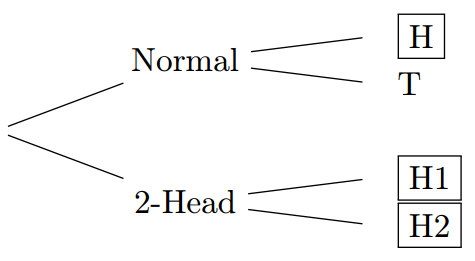
\includegraphics{2headedcoin1.png}
%\begin{tikzpicture}[grow=right]
%\tikzstyle{level 1}=[level distance=2cm, sibling distance=1.5cm]
%\tikzstyle{level 2}=[level distance=2cm, sibling distance=.5cm]
%\node{}
%    child {
%    	node[] {2-Head}
%        	child {
%            	node[label=right:{\boxed{\text{H2}}}] {}
%                edge from parent
%            }
%            child {
%            	node[label=right:{\boxed{\text{H1}}}] {}
%                edge from parent
%            }
%        edge from parent
%    }
%    child {
%    	node[] {Normal}
%        	child {
%            	node[label=right:{T}] {}
%                edge from parent
%            }
%            child {
%            	node[label=right:{\boxed{\text{H}}}] {}
%                edge from parent
%            }
%        edge from parent
%    };
%\end{tikzpicture}
\end{image}

Notice that there are three equally likely outcomes where we see a head and two of them correspond to the 2-headed coin. This means that the probability that we have picked the two-headed coin is $\frac{2}{3}$.

\begin{question}
If your friend flips the coin and gets another head, what's the probability that you chose the two-headed coin? (Give your answer as decimal.)

    \answer{$0.8$}
    \begin{hint}
      Draw the probability tree. Start from the one above (draw it without boxes) and extend it one more level.
    \end{hint}
    \begin{hint}
      The ways you can see two heads in a row are H-H, H1-H1, H1-H2, H2-H1, and H2-H2.
    \end{hint}

\end{question}

So you can see that the information that you are receiving from your friend is giving you higher levels of confidence in your conclusion. It's important to note that you can never conclusively conclude that the coin is two-headed using this technique. There will always be a small chance that the flips of a fair coin will randomly land on heads many heads in row.

\end{document}